% What the simulation covers, and where it stops. Cascade drawn against a
% logarithmic time axis, after the event-display idiom: a hard event, a
% branching development, and a legend for the species.
% Compile from `docs/preprint`:  lualatex sekil/kaskad.tex
\documentclass[border=3pt,tikz]{standalone}
\usepackage{amsmath}
\usepackage[outline]{contour}
\usetikzlibrary{calc,arrows.meta,shapes.geometric,decorations.pathmorphing,
                decorations.markings,patterns}
\contourlength{1.0pt}
\tikzset{>=latex}

\colorlet{ink}{black!82}
\colorlet{gh}{black!40}
\colorlet{impcol}{red!75!black}
\colorlet{shockcol}{violet!65!black}
\colorlet{digcol}{brown!65!black}
\colorlet{conecol}{orange!88!black}
\colorlet{freecol}{blue!55!cyan!75!black}
\colorlet{backcol}{red!72!black}
\colorlet{boundcol}{orange!60!black}

\begin{document}
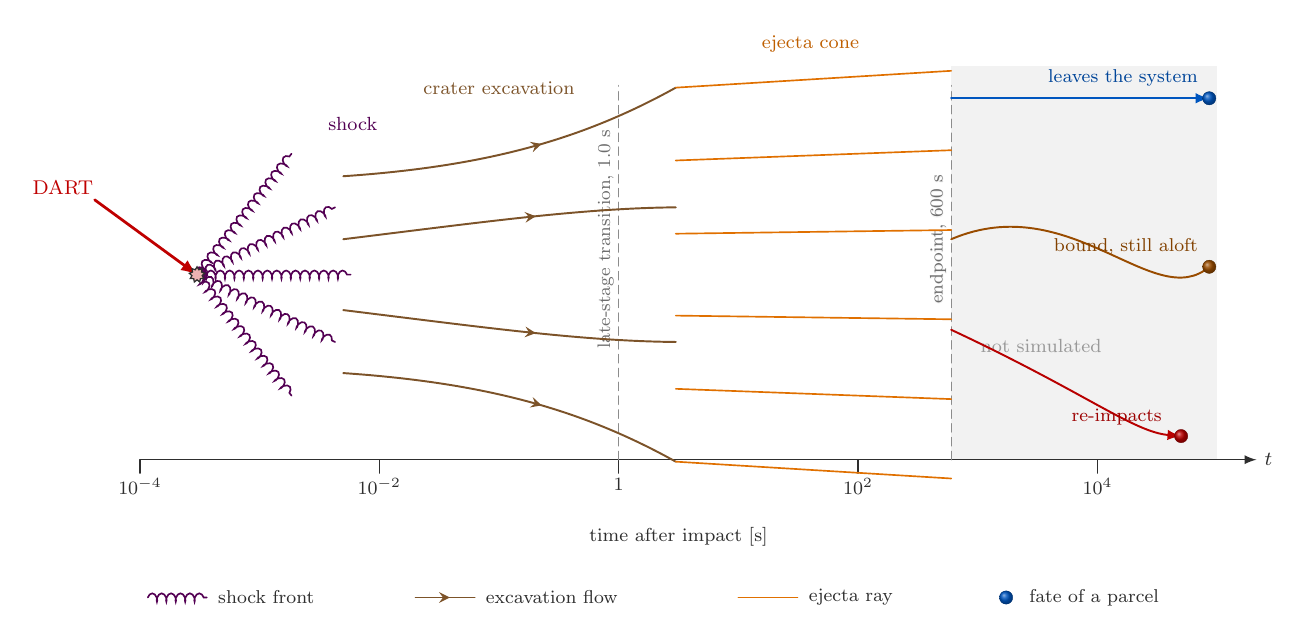
\begin{tikzpicture}[
  font=\footnotesize, line cap=round,
  thin_/.style={line width=0.35pt, draw=gh},
  shock/.style={decorate, draw=shockcol, line width=0.6pt,
    decoration={coil, amplitude=1.5pt, segment length=3.4pt}},
  flow/.style={draw=digcol, line width=0.7pt,
    postaction={decorate, decoration={markings,
      mark=at position 0.58 with {\arrow[draw=digcol]{stealth}}}}},
  ray/.style={draw=conecol, line width=0.6pt},
  ball/.style={draw=none, ball color=#1, postaction={fill=#1,
    fill opacity=0.35, draw=#1!60!black, line width=0.12}},
  ball/.default=conecol,
]

% x maps log10(t/s) to centimetres; t from 1e-4 s to 1e5 s
\pgfmathsetmacro{\XL}{-4} \pgfmathsetmacro{\XR}{5}
% Argument is log10(t/s): see scripts note. pgfmath cannot take
% the logarithm of a number this small itself.
\newcommand{\X}[1]{{(#1-(\XL))*1.52}}
\pgfmathsetmacro{\W}{((\XR)-(\XL))*1.52}

% ---------- the region we do not simulate ------------------------------
\fill[ink!6] (\X{2.7782},-2.35) rectangle (\W,2.65);
\node[gh, scale=0.86, anchor=north west, align=left]
     at (\X{2.9542},-0.72) {not simulated};

% ---------- time axis ---------------------------------------------------
\draw[->, ink, line width=0.5pt] (0,-2.35) -- (\W+0.5,-2.35)
     node[anchor=west, scale=0.9, inner sep=3pt] {$t$};
\foreach \e/\lab in {-4/{$10^{-4}$}, -2/{$10^{-2}$}, 0/{$1$},
                     2/{$10^{2}$}, 4/{$10^{4}$}}{
  \pgfmathsetmacro{\xx}{(\e-(\XL))*1.52}
  \draw[ink, line width=0.5pt] (\xx,-2.35) -- (\xx,-2.52)
       node[below, scale=0.85, text=ink, inner sep=2pt] {\lab};
}
\node[ink, scale=0.85, anchor=north] at (\W/2,-3.1) {time after impact [s]};

% ---------- the two locked model times ---------------------------------
\draw[densely dashed, ink!55, line width=0.5pt] (\X{0.0000},-2.35) -- (\X{0.0000},2.4);
\node[ink!70, scale=0.82, rotate=90, anchor=south, inner sep=2pt]
     at (\X{0.0000},0.45) {\contour{white}{late-stage transition, $1.0$ s}};
\draw[densely dashed, ink!55, line width=0.5pt] (\X{2.7782},-2.35) -- (\X{2.7782},2.4);
\node[ink!70, scale=0.82, rotate=90, anchor=south, inner sep=2pt]
     at (\X{2.7782},0.45) {\contour{ink!6}{endpoint, $600$ s}};

% ---------- the impact ---------------------------------------------------
\coordinate (I) at (\X{-3.5229},0);
% `\X` expands to a braced group, so arithmetic cannot be appended to it
% inside a coordinate; an earlier time value gives the same offset.
\draw[impcol, line width=1.0pt, ->] (\X{-4.3778},0.95) -- (I);
\node[impcol, scale=0.9, anchor=south east, inner sep=2pt]
     at (\X{-4.3449},0.95) {DART};


% ---------- shock ---------------------------------------------------------
\foreach \a in {-52,-26,0,26,52}{
  \draw[shock] (I) -- ++(\a:1.95);
}
\node[star, star points=9, draw=ink, line width=0.45pt,
      fill=impcol!30, inner sep=1.4pt, scale=0.95] at (I) {};
\node[shockcol, scale=0.86, anchor=south] at ({\X{-2.2218}},1.72)
     {\contour{white}{shock}};

% ---------- excavation flow ----------------------------------------------
\foreach \y/\c in {-1.25/1.1, -0.45/1.5, 0.45/1.5, 1.25/1.1}{
  \draw[flow] ({\X{-2.3010}},\y) .. controls ({\X{-1.0969}},{\y*\c}) and
      ({\X{-0.3010}},{\y*\c*1.25}) .. ({\X{0.4771}},{\y*1.9});
}
\node[digcol, scale=0.86, anchor=south] at ({\X{-1.0000}},2.18)
     {\contour{white}{crater excavation}};

% ---------- ejecta cone ---------------------------------------------------
% Start where the excavation flows end, otherwise the cascade has a
% visible gap in the middle.
\foreach \y in {-2.375,-1.45,-0.52,0.52,1.45,2.375}{
  \draw[ray] ({\X{0.4771}},\y) -- ({\X{2.7782}},{\y*1.09});
}
\node[conecol!85!black, scale=0.86, anchor=south] at ({\X{1.6021}},2.72)
     {\contour{white}{ejecta cone}};

% ---------- the three fates ----------------------------------------------
\draw[freecol, line width=0.7pt, ->] ({\X{2.7782}},2.24) -- (\W-0.1,2.24);
\draw[boundcol, line width=0.7pt] ({\X{2.7782}},0.45) .. controls
     ({\X{3.7782}},1.1) and ({\X{4.4771}},-0.5) .. (\W-0.1,0.1);
\draw[backcol, line width=0.7pt, ->] ({\X{2.7782}},-0.7) .. controls
     ({\X{3.9031}},-1.5) and ({\X{4.3010}},-2.0) .. ({\X{4.6990}},-2.05);

\draw[ball=freecol]  (\W-0.1,2.24) circle (2.4pt);
\draw[ball=boundcol] (\W-0.1,0.1) circle (2.4pt);
\draw[ball=backcol]  ({\X{4.6990}},-2.05) circle (2.4pt);

\node[freecol!80!black, scale=0.84, anchor=south east, inner sep=3pt]
     at (\W-0.15,2.3) {leaves the system};
\node[boundcol!85!black, scale=0.84, anchor=south east, inner sep=3pt]
     at (\W-0.15,0.16) {bound, still aloft};
\node[backcol!85!black, scale=0.84, anchor=south east, inner sep=3pt]
     at (\X{4.5999},-2.0) {re-impacts};

% ---------- legend --------------------------------------------------------
\begin{scope}[shift={(0.1,-4.1)}]
  \draw[shock] (0,0) -- (0.75,0);
  \node[ink, scale=0.84, anchor=west, inner sep=3pt] at (0.8,0)
       {shock front};
  \draw[flow] (3.4,0) -- (4.15,0);
  \node[ink, scale=0.84, anchor=west, inner sep=3pt] at (4.2,0)
       {excavation flow};
  \draw[ray] (7.5,0) -- (8.25,0);
  \node[ink, scale=0.84, anchor=west, inner sep=3pt] at (8.3,0)
       {ejecta ray};
  \draw[ball=freecol] (10.9,0) circle (2.4pt);
  \node[ink, scale=0.84, anchor=west, inner sep=3pt] at (11.1,0)
       {fate of a parcel};
\end{scope}

\end{tikzpicture}
\end{document}
